\chapter{Schreiben der Compiler}

\section{THS Compiler}
Der THS Compiler folgt dem theoretischen Aufbau eines Compilers und besteht aus Lexer, Parser und Code Generator. Als Parser wird ein Predictive Descent Parser verwendet.
Der Code Generator arbeitet auf dem Abstract Syntax Tree mithilfe eines Visitor Patterns. Die Semantic Analysis wird während der Code Generation durchgeführt. Geschrieben ist der Compiler in C++ und liefert x86 Assembly nach NASM Syntax.

\section{QHS Compiler}
Genauso wie der THS Compiler ist auch der QHS Compiler in C++ geschrieben und generiert x86 Assembly nach NASM Syntax.
Jedoch unterscheiden sich beide Compiler stark in der Funktionsweise. Der Compilation von QHS steht ein einfacher Zyklus zugrunde, dessen Vorbild der Von-Neumann Zyklus ist.

\begin{figure}[h!]
    \centering
    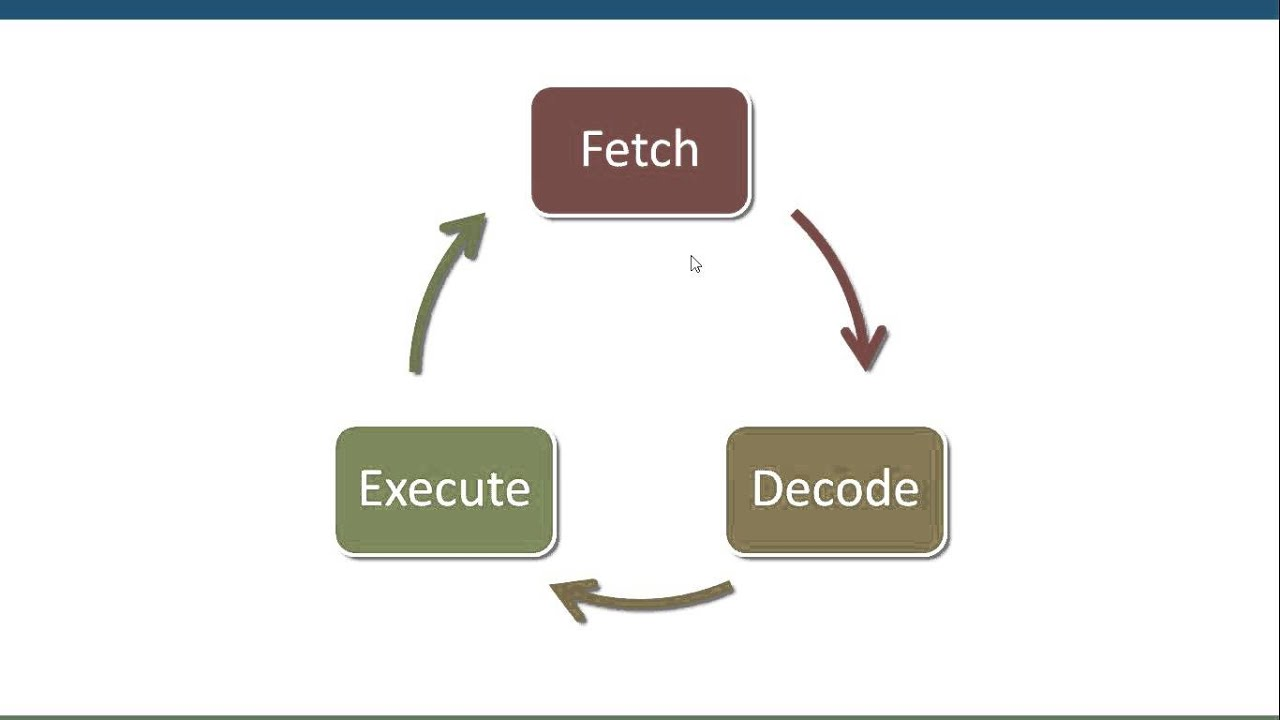
\includegraphics[scale=0.3]{resources/TEMP_von-neumann-cycle.jpg}
    \caption{TEMP! Zyklus der QHS Compilation, basierend auf Von-Neumann Zyklus}
    \label{fig:von-neumann-cycle}
\end{figure}

TALK ABOUT ORDERS AND THE MEANING OF IDENTIFIERS, INSTRUCTIONS AND LITERAL CODE

\subsection{Fetch}
Der QHS-Zyklus beginnt mit dem ersten Fetch. Dabei wird die erste Order aus dem Inputfile extrahiert. Eine Order weist einen der drei Typen Identifier, Instruction oder Literal-Code auf. Diese sind mit folgenden RegEx definiert.

\begin{table}[h]
    \centering
    \begin{tabular}{ll}
    \multicolumn{1}{l|}{identifier}        & \textless{}identiferChar\textgreater{}*                           \\ \hline
    \multicolumn{1}{l|}{instruction}       & \# \textless{}identiferChar\textgreater{}*                        \\ \hline
    \multicolumn{1}{l|}{literalCode}       & ".*"                                                              \\
                                           &                                                                   \\
    \textless{}identiferChar\textgreater{} & = {[}\textasciicircum{}\# "\textless{}whitespace\textgreater{}{]} \\
    \textless{}whitespace\textgreater{}    & = SPACE | NEWLINE | TAB
    
    \end{tabular}
\end{table}

Ist die Order vom Typ Identifier oder Literal-Code, wird diese sofort an den nächsten Schritt im Zyklus Decode weitergegeben. Handelt es sich jedoch um eine Instruction ist es dieser möglich hier in den Zyklus einzugreifen.
Bestimmte Instructions ignorieren die Decode und Execute Schritte und fahren mit dem nächsten Fetch fort, andere geben anstelle von sich selbst eine andere Order an Decode weiter. Auch ist es möglich nur Decode zu überspringen und
direkt Execute auszuführen. Wie und ob eine Instruction in den Zyklus eingreift, lässt sich im QHS Compiler frei definieren.

Weiter ist es möglich zu beeinflussen Orders \textbf{voraus zu stellen}, die anstelle der nächsten Order im Inputfile gefetched werden. Dies geschieht mit Hilfe des Fetch-Stacks auf den eine Liste an Orders gepushed werden kann.
Dieser Fetch-Stack folgt Last-In First-Out und \textbf{auf ihn} kann während jeder der drei Schritte des Zyklus gepushed werden. Die Hauptanwendung des Fetch-Stacks wird im Abschnitt \ref{sec:qhs-execute} ausgeführt.

\begin{figure}[h!]
    \centering
    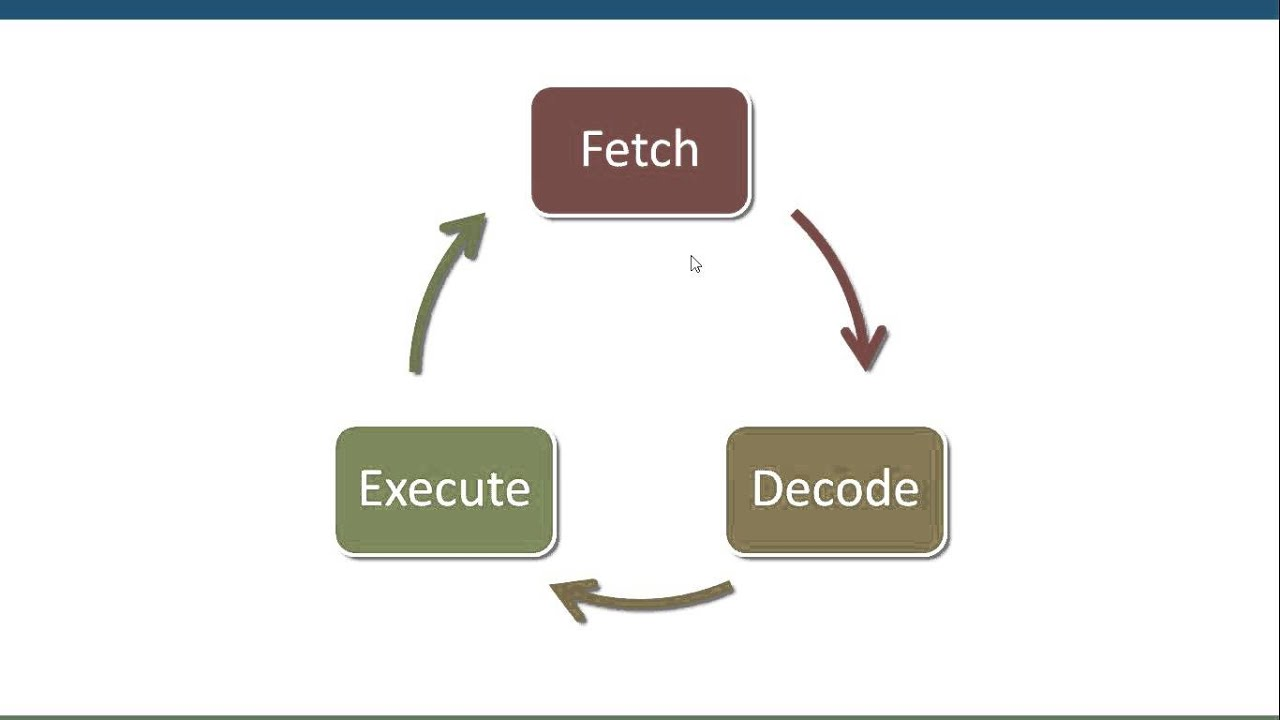
\includegraphics[scale=0.3]{resources/TEMP_von-neumann-cycle.jpg}
    \caption{TEMP! Struktur des Fetch-Stacks}
    \label{fig:fetch-stack}
\end{figure}

Wenn eine Liste an Orders komplett gefetched wurde, wird diese vom Stack gelöscht. Der Inputfile befindet sich auf dem letzten Platz des Fetch-Stacks und wird somit nur verwendet, wenn der Stack ansonsten komplett leer ist.
Die Compilation wird beendet, sobald keine Order mehr auf dem Fetch-Stack übrig ist.

\subsection{Decode} \label{sec:qhs-decode}
Nachdem eine Order gefetched wurde, wird diese an Decode weitergegeben. \textbf{Während Decode werden zwei Aufgaben durchgeführt}.
Als erstes geht es darum Orders des Typen Identifier ihrer jeweiligen Definition zuzuortnen, sowie auf undefinierte Identifier hinzuweisen und diese zu überspringen.

MAYBE TALK ABOUT ENVIRONMENTS

Als zweites kommt während dem Decode Schritt der Order-Stack ins Spiel. Hierbei handelt es sich um die gleiche Datenstruktur wie der Fetch-Stack. Jedoch ist dessen Anwendung nicht das Vorausstellen von Orders vor den Inputfile,
sondern das Speichern und spätere Ausführen von Orders. Der Order-Stack kann mit Hilfe von Instructions, die im Abschnitt \ref{sec:qhs-execute} weiter ausgeführt werden, aktiviert und deaktiviert werden.
Bei der Aktivierung wird eine leere Liste, die nach First-In First-Out aufgebaut ist, auf den Order-Stack gepushed. Wenn nun eine Order in den Decode Schritt gelangt und der Order-Stack aktiviert ist,
wird diese Order der momentan obersten Liste des Order-Stacks hinzugefügt. Der Execute Schritt wird danach übersprungen und der Zyklus beginnt von neuem bei Fetch. Die Order wurde ohne ausgeführt zu werden auf dem Order-Stack gespeichert.
Später ist es nun möglich diese Order mit Hilfe von Instructions, die im Abschnitt \ref{sec:qhs-execute} weiter thematisiert werden, vom Order-Stack zu enfernen und auszuführen.
Bestimmte Instructions und Identifiers können jedoch Order-Stack-Proof, also immun gegen den Order-Stack, gemacht werden. Diese werden, auch wenn der Order-Stack aktiv ist, normal an Execute weitergegeben.
Dies ist zum Beispiel besonders bei der Instruction, die den Order-Stack wieder deaktiviert, wichtig. Da diese sonst nicht ausgeführt und somit der Order-Stack niemehr deaktiviert wird.
LiteralCode kann nicht Code-Stack-Proof sein.

Ist der Order-Stack deaktiviert oder die Order Code-Stack-Proof wird diese an den letzen Schritt Execute weitergegeben.

\subsection{Execute} \label{sec:qhs-execute}